\chapter{Background}
\label{chapt:bg}

This thesis draws upon
what would traditionally be thought of a disparate fields:
phonetics and phonology from linguistics,
psychoacoustics from psychology,
knowledge representation
and artificial neural networks from computer science,
spiking neural networks
from computational neuroscience,
and dynamical systems and control theory
from systems design engineering.
For clarity, the background presented
in this chapter is limited
to subjects specifically related to speech.
I assume basic knowledge in
computer science or engineering,
but will review the specific techniques
used in this thesis
in Chapter~\ref{chapt:methods}.

\section{Speech perception \& recognition}

On the sensory side of speech,
we aim to apply aspects of speech perception
to automatic speech recognition (ASR)
in order to
improve the performance of ASR systems,
and make progress toward
the long-term goal of a closed-loop
computational speech system
that recognizes and synthesizes speech
in a single interconnected network.
In this section,
we review fundamental concepts and literature
in basic ear physiology,
psychoacoustics,
auditory neurobiology,
and automatic speech recognition.

\subsection{Ear physiology}

The human ear transduces fluctuations in
air pressure level to neural signals
that we interpret as sounds.
It does this by mechanically
separating the air pressure level fluctuations
into instantaneous frequency components,
which is the basic representation
that the brain receives.
Figure~\ref{fig:an-overview} illustrates
the major structures involved
in sound transduction.

\fig{an-overview}{0.8}{Overview of the human ear.}{
  Overview of the human ear. Fluctuations in air pressure
  travel down the auditory canal
  and cause the tympanic membrane to vibrate.
  These vibrations result in a tiny bone
  called the stapes rapidly moving
  in and out of the oval window of the cochlea.
  The disturbances of the liquid in the cochlea
  deflect the basilar membrane inside,
  with high frequency disturbances
  causing deflections at the base of the cochlea,
  and low frequency disturbances causing deflections
  at the apex of the cochlea.
  Electrical activity in the form of action potentials
  are produced in the cochlea,
  and enter the brain through the cochlear nerve.
  Adapted from \citet{chittka2005}.}

The outer ear (pinna) funnels air
into the ear canal,
and modifies the air pressure wave
such that the directionality
of sound can be determined.
In the middle ear,
air pressure fluctuations
cause the eardrum (tympanic membrane)
to vibrate;
these minuscule vibrations
cause three tiny bones,
the malleus, incus, and stapes to move.
The stapes sits on the oval window
of the cochlea,
such that when the eardrum vibrates,
the stapes moves in and out of the oval window,
causing disturbances in the liquid
in the cochlea
(see Figure~\ref{fig:cochlea}).
Importantly for modeling,
the external and middle ear
also attenuate low frequency sounds
and amplify mid frequency sounds
(2--7 kHz)
\citep{rosowski1996,ballachanda1997}.

\fig{cochlea}{0.55}{Cochlea cross-section.}{
  Cross-section of the cochlea.
  As the basilar membrane deflects
  due to the motion of the stapes
  in and out of the oval window of the cochlea,
  inner hair cells are pushed against
  the tectorial membrane.
  When deflected,
  the stereocilia on the top of the hair cells
  allow positive charged ions to enter
  the cell.
  The change in inner hair cell voltage
  causes action potentials to fire in
  spiral ganglion cells,
  which travel down
  the cochlear (auditory) nerve.
  Outer hair cells are attached to
  the tectorial membrane,
  and act as a dynamic amplifier
  (see text for more details).
  Adapted from \citet{kandel2000}.}

The inner ear transduces vibrations
of the liquid in the cochlea
to electrical signals transmitted
to the brain.
As liquid in the cochlea
moves past the basilar membrane,
it causes it to deflect
based on the width and thickness
of the membrane at that point
in the cochlea.
The basilar membrane
is shaped such that
the base of the membrane
(near the stapes)
is deflected when
incoming vibrations have power
at high frequencies,
up to 20,000~Hz.
The membrane becomes sensitive
to lower and lower frequencies
going further down the membrane
to the apex
in the center of the cochlea,
which is deflected when incoming vibrations
have power as low as 20~Hz.

The basilar membrane's surface is covered
with hair cells that transduce
the deflections of the membrane
to electric current.
Stereocilia on the top of inner hair cells
rests on or near the tectorial membrane
(see Figure~\ref{fig:cochlea}).
When the basilar membrane deflects,
the stereocilia's orientation
relative to the tectorial membrane changes,
which mechanically opens receptors
on top of the stereocilia,
allowing positive charged ions
(mostly potassium and calcium)
to enter the hair cell.
Inner hair cells synapse with
spiral ganglion cells,
which accumulate the continuously
changing voltage of the inner hair cells
and send action potentials
down the auditory nerve
conveying how much power
is present at the current moment
at the frequency characteristic
of that section of the basilar membrane.
Outer hair cells play a more nuanced
role in transduction.
Their activity is tuned
more broadly in both space and time,
and seem to act as a dynamic amplifier,
amplifying quiet sounds and
attenuating loud sounds
\citep{dallos1992}.
This dynamic amplification allows
the human ear to have a wide dynamic range,
able to safely hear sounds from 0--130~dB,
which represents 13 orders of magnitude
of absolute air pressure.

\subsection{Psychoacoustics}
\label{sec:psychoacoustics}

Psychoacoustics provides a quantitative account
of how the human auditory system
responds to incoming air pressure levels.
In this thesis, we review psychoacoustics
under the assumption that
the human auditory system
has evolved to be adept at processing speech.
While the human ear can be thought of
as a spectrum analyzer for air pressure waves,
there are important differences between
a straightforward Fourier analysis
and how the ear and early auditory brain regions
respond to air pressure waves.
Assuming that the human
auditory system has evolved to be
well-suited for speech,
it stands to reason that
capturing these differences
is important for speech recognition.
Therefore, the psychoacoustical findings
discussed in this chapter
are presented as motivation for the
auditory periphery models described
in Section~\ref{sec:periphery-models}.

\subsubsection{Spatial psychoacoustical effects}

Sound pressure levels can be objectively measured
and expressed in terms of the logarithmic
decibel (dB) scale.
Human perception of loudness can help
determine the transfer functions
at different parts of the auditory system.
Early studies investigated
subjective loudness in response
to pure tones,
as tones of equal objective volume
are perceived as louder for higher frequencies.
The exact relationship between
sound pressure level and
loudness was originally proposed
by \citet{fletcher1933},
and further standardized
by the international standards organization
(ISO-226:2003);
see Figure~\ref{fig:el-curves}.
In general, perceived loudness,
as expressed in the phon scale,
increases for higher frequency sounds
up to around 7000~Hz.

\fig{el-curves}{0.65}{Equal loudness curves.}{
  Equal loudness curves.
  Each line denotes a contour
  of equal subjective loudness
  for a loudness level given in units of phon
  (determined empirically through many studies,
  beginning with \citealt{fletcher1933}).
  Generally, low frequency sounds must have higher
  sound pressure levels to reach the same loudness
  as sounds with lower pressure at higher frequencies.}

Another scale, the sone,
quantifies the relative differences
to pure tones played with
different sound pressure levels.
Specifically, the sone scale
is linear with perceived loudness;
a sound played with twice the sone value
should be perceived as twice as loud.
The sone for a particular frequency is
\begin{equation*}
  \text{sone} \approx 2^{\frac{\text{phon} - 40}{10}},
\end{equation*}
above signals of 40~phon or louder.

The difference in perceived loudness
across the frequency spectrum,
along with the organization
of the inner ear,
suggests that a better model
of the ear (instead of as a spectrum analyzer)
is as a bank of narrowband filters.
Support for this model was provided
in \citet{zwicker1957},
who showed that when two tones
have frequencies that are close enough,
their perceived loudness sums,
suggesting that the two tones
are within the bandwidth of one of the
auditory system's filters.
\citet{moore1983}
summarized other attempts to
determine the bandwidth
of auditory filters
in a simple equation
describing the equivalent
rectangular bandwidth (ERB)
of auditory filters:
\begin{equation*}
  \text{ERB} = 6.23 f^2 + 93.39 f + 28.52,
\end{equation*}
where $f$ is the center frequency
of the auditory filter of interest.
See Figure~\ref{fig:erb-mel} for a visualization of
this measure for frequencies of relevance
for the human auditory system.
Auditory filters are not rectangular,
but for simplification this equation
treats them as such;
despite this simplification,
the ERB measure has been productive and is still used
to determine the bandwidths
of filters in auditory periphery models.

\fig{erb-mel}{0.65}{Equivalent rectangular bandwidth (ERB) and Mel scales.}{
  Two scales based on psychoacoustic experiments
  quantifying perception of sounds of different frequencies.
  The equivalent rectangular bandwidth scale
  (ERB; \citealp{moore1983}),
  plotted in blue,
  summarizes the bandwidth of auditory filters
  at different frequencies.
  The Mel scale \citep{stevens1937},
  plotted in green,
  summarizes the perceived pitch
  for the given frequency.}

Like volume,
humans perceive
the frequency of incoming sounds
in subjective ways.
The subjective perception of frequency
is referred to as pitch.
\citet{stevens1937} quantified
the relationship between
frequency and pitch
with a simple equation,
\begin{equation*}
  \text{Mel} = 2595 \log_{10} \left(1 + \frac{f}{700}\right),
\end{equation*}
resulting in the Mel scale
(see Figure~\ref{fig:erb-mel}).
As with volume, humans are adept at
noticing when two tones differ in pitch;
however, absolute perceptions of pitch
have far less granularity
(musical notation, for example,
uses seven degrees of pitch per octave
and seven degrees of loudness).

\subsubsection{Temporal psychoacoustical effects}

To this point, we have discussed
spatial psychoacoustical effects,
which depend on
the sound pressure level
at a moment in time.
There are also several temporal effects
which are important for speech.
The first is that the length
of a sound affects its perceived volume.
Specifically, short sounds are harder to hear
(see Figure~\ref{fig:short-sounds}).
As a result, humans find
consonant sounds more difficult
to recognize in situations with background noise
than vowel sounds,
as consonants are shorter than vowels
\citep[Chapter~3]{everest2001}.
There is evidence that sounds with constant volume
are perceived as being monotonically louder
up to approximately 200~ms;
this finding suggests that
at some point in the auditory system,
the power for a given characteristic frequency
is integrated over a time window
of approximately 200~ms
\citep[p.64]{kollmeier2008}.

\fig{short-sounds}{0.65}{Short sounds are less audible than longer ones.}{
  When audio samples are played for shorter durations,
  they are perceived as quieter,
  for both random noise and pure tone samples.
  Perceived loudness can be equalized
  by raising the sound pressure level of the audio pulse;
  the relationship between
  how much the sound pressure level must be raised
  and the duration of the audio sample
  is plotted.
  Adapted from \citet[p.60]{everest2001}.}

Another temporal effect is forward and backward masking.
When two sounds are made in quick succession,
the louder sound of the two can
``mask'' the quieter sound,
rendering it inaudible,
even though it would be audible
were it made in isolation.
When the masked (quieter) sound
precedes the masker (louder sound),
it is called backward masking;
the reverse is called forward masking.
Spatial masking also occurs
when two sounds differ in loudness,
and are within the bandwidth
of an auditory filter.

Our perception of echoes can also tell us
something about how the auditory system
responds to temporally transformed sounds.
We perceive all sounds arriving within
a certain time window as occurring at essentially
the same time;
for example, in an enclosed room,
we hear our own speech as we voice it,
and shortly thereafter when it is reflected
back to us off of the walls.
Yet, we perceive this as a single utterance,
a phenomenon known as auditory fusion.
\citet{haas1972} found that auditory fusion occurs
best when similar sounds are separated by roughly
20 to 30~milliseconds.
When similar sounds are separated by 50 to 80~milliseconds,
we perceive them as discrete echoes.

Together, these temporal psychoacoustical effects
suggest that the incoming frequency information
from the filters implemented by the auditory periphery
are further temporally filtered
by auditory regions of the brain.

\subsection{Linguistics}
\label{sec:perc-linguistics}

Following psychoacoustics,
linguistics provides
the next level of insight into
how we perceive speech.
While a full treatment of linguistics
is impossible in this short space,
we will briefly introduce
key concepts in phonology,
phonetics, morphology, and semantics
in order to
explain the speech perception hierarchy
summarized in Figure~\ref{fig:perception}.\footnote{
  When not explicitly cited,
  the information in Sections~\ref{sec:perc-linguistics}
  and \ref{sec:prod-linguistics}
  should be considered
  basic linguistics
  that would be covered in an
  introductory undergraduate level
  class or textbook
  (I used \citet{roach2010} as a general reference).
}\footnote{The International Phonetic Alphabet (IPA)
  will be used this and subsequent sections.
  See Figure~\ref{fig:vowels} and Table~\ref{tab:consonants}
  for more details.}

\fig{perception}{0.2}{Hierarchy of linguistic concepts in speech perception.}{
  Hierarchy of linguistic concepts in speech perception.
  A continuous audio signal contains
  a string of discrete phones,
  which are processed in a linguistic context
  to yield a string of phonemes.
  A morpheme is composed of one or more phonemes,
  and a word is composed of one or more morphemes.
  While there are further levels
  in the speech perception hierarchy,
  we limit our discussion to the levels
  up to words.}

\subsubsection{Phones \& phonemes}

The smallest linguistically relevant unit
is the phoneme, which conceptually
summarizes the linguistically relevant
aspects of a phone,
which is a short speech sound
on the order of tens of milliseconds.
Phonemes are noted by their ability
to change the meaning of some word
when swapped in speech;
for example, the only difference between
the word ``bad'' and ``mad'' is the
consonant phoneme
at the beginning
(\ipa{/b/} or \ipa{/m/}).
Phones, on the other hand,
describe the actual sounds
produced by a speaker.
The repository of all possible phones
is therefore larger than the phonemes
used in a particular language.
More than one phone can map
to a phoneme;
for example, the English word
``pin'' can be voiced as
\ipa{[pIn]} or \ipa{[p\super{h}In]}
and will be recognized by
all English speakers
as \ipa{/pIn/} because
the \ipa{[p\super{h}]} phone
is used interchangeably with
\ipa{[p]} in English
(i.e., \ipa{[p\super{h}]} and \ipa{[p]}
are allophones).

Even though different individuals
voice each phone differently,
the important quality is that
the particular sound is perceived
as a particular phoneme
by a listener
in the context of an utterance.
A helpful analogy can be made between
phones in speech
and alphabetical letters in writing.
With no knowledge of English,
seeing the sentence,
``A bird has a wing,''
one might think that ``A'' and ``a''
are different letters.
However, with enough examples,
one could surmise that in every situation
where ``A'' is used, it appears at the
start of a sequence of letters,
and it could have instead
been replaced by ``a''
had it not appeared at the start of the sequence.
Therefore, ``A'' and ``a'' represent
the same underlying ``letter.''
Similarly, despite individual differences
in the pitch, speed, volume, and quality
of how one realizes a particular phoneme,
that realization is still considered the same
if it plays the same role
in a linguistically relevant sequence of phonemes.
Accents come about, in part,
because different languages use different
sets of phonemes,
and adults have difficulty
learning to perceive and produce
phones not encountered early in life.

While there are many properties
of phones and phonemes,
in this thesis we are only concerned
with whether it
is a vowel or a consonant.
Vowels are longer sounds
made when the vocal tract is mostly open.
Consonants are shorter sounds
made when some part of the vocal tract
is constricted or transiently closed.
In almost all languages,
there are more consonant phonemes
than there are vowel phonemes,
though pronunciation varies significantly
between dialects,
and transcribing the full set of
phonemes in a language is
not a purely objective exercise.

Vowel phones occur when air is freely
moving through the open vocal tract.
The shape of the vocal tract determines
the quality of the sound.
Three factors influence vowel vocal tract shape:
openness, backness, and roundedness.
Openness refers to the general position
of the jaw (open or closed) and tongue (low or high);
backness refers to the position of the
tongue relative to the back of the mouth;
and roundedness refers to
whether the lips are rounded.
Roundedness can vary independently
of the other factors;
therefore, each vowel sound has a rounded
and unrounded variant.
Openness and backness are partially coupled,
such that when the vocal tract is open,
it must be mostly (but not completely) back.
The three possible extremes, then,
are \ipa{[A]} (open, back),
\ipa{[i]} (closed, front),
and \ipa{[u]} (closed, back).
Most of the remaining vowel sounds
can be expressed as being
a blend of one of these three vowel sounds
(see Figure~\ref{fig:vowels} for a visualization).

The frequency spectrum of vowel sounds
typically shows three frequencies
of relatively high power,
which are called formants.
In most cases, the first two formants
(i.e., the lower two frequencies)
are sufficient to disambiguate
between vowel phones.

\begin{figure}[ht!]
  \centering
  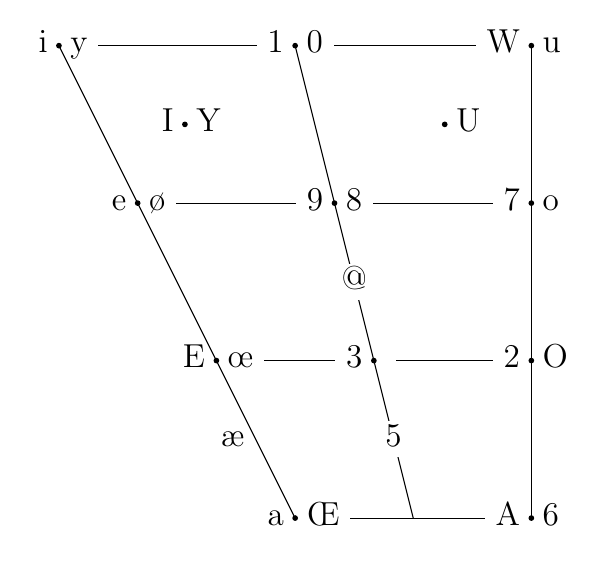
\begin{tikzpicture}[scale=3]
    \large
    \tikzset{
      vowel/.style={fill=white, anchor=mid, text depth=0ex, text height=1ex},
      dot/.style={circle,fill=black,minimum size=0.4ex,inner sep=0pt,outer sep=-1pt},
    }
    \coordinate (hf) at (0,2); % high front
    \coordinate (hb) at (2,2); % high back
    \coordinate (lf) at (1,0); % low front
    \coordinate (lb) at (2,0); % low back
    \def\V(#1,#2){barycentric cs:hf={(3-#1)*(2-#2)},hb={(3-#1)*#2},lf={#1*(2-#2)},lb={#1*#2}}

    % Draw the horizontal lines first.
    \draw (\V(0,0)) -- (\V(0,2));
    \draw (\V(1,0)) -- (\V(1,2));
    \draw (\V(2,0)) -- (\V(2,2));
    \draw (\V(3,0)) -- (\V(3,2));

    % Place all the unrounded-rounded pairs next, on top of the horizontal lines.
    \path (\V(0,0))     node[vowel, left] {\ipa{i}} node[vowel, right] {\ipa{y}} node[dot] {};
    \path (\V(0,1))     node[vowel, left] {\ipa{1}} node[vowel, right] {\ipa{0}} node[dot] {};
    \path (\V(0,2))     node[vowel, left] {\ipa{W}} node[vowel, right] {\ipa{u}} node[dot] {};
    \path (\V(0.5,0.4)) node[vowel, left] {\ipa{I}} node[vowel, right] {\ipa{Y}} node[dot] {};
    \path (\V(0.5,1.6)) node[vowel, left] {} node[vowel, right] {\ipa{U}} node[dot] {};
    \path (\V(1,0))     node[vowel, left] {\ipa{e}} node[vowel, right] {\ipa{\o}} node[dot] {};
    \path (\V(1,1))     node[vowel, left] {\ipa{9}} node[vowel, right] {\ipa{8}} node[dot] {};
    \path (\V(1,2))     node[vowel, left] {\ipa{7}} node[vowel, right] {\ipa{o}} node[dot] {};
    \path (\V(2,0))     node[vowel, left] {\ipa{E}} node[vowel, right] {\ipa{\oe}} node[dot] {};
    \path (\V(2,1))     node[vowel, left] {\ipa{3}} node[vowel, right] {\ipa{\textcloseepsilon}} node[dot] {};
    \path (\V(2,2))     node[vowel, left] {\ipa{2}} node[vowel, right] {\ipa{O}} node[dot] {};
    \path (\V(2.5,0))   node[vowel, left] {\ipa{\ae}} node[vowel, right] {} node[   ] {};
    \path (\V(3,0))     node[vowel, left] {\ipa{a}} node[vowel, right] {\ipa{\OE}} node[dot] {};
    \path (\V(3,2))     node[vowel, left] {\ipa{A}} node[vowel, right] {\ipa{6}} node[dot] {};

    % Draw the vertical lines.
    \draw (\V(0,0)) -- (\V(3,0));
    \draw (\V(0,1)) -- (\V(3,1));
    \draw (\V(0,2)) -- (\V(3,2));

    % Place the unpaired symbols last, on top of the vertical lines.
    \path (\V(1.5,1))   node[vowel]       {\ipa{@}};
    \path (\V(2.5,1))   node[vowel]       {\ipa{5}};
  \end{tikzpicture}
  \caption[Vowels defined in the IPA.]{Vowels defined in the
    International Phonetic Alphabet (IPA),
    organized along three axes.
    The vertical axis reflects whether the vocal tract
    is open or closed.
    The horizontal axis reflects whether the tongue
    is near the front or back of the mouth.
    The last axis, on either side of each dot ($\cdot$)
    reflects whether the lips are rounded or unrounded.}
\label{fig:vowels}
\end{figure}

Consonant phones occur when some point
of the vocal tract is constricted.
The place and manner of constriction
determines the consonant that will be uttered.
Place refers to the location in the vocal tract
that becomes constricted.
For example, in bilabial consonants,
both lips come together,
as in \ipa{[m]} and \ipa{[b]};
in velar consonants,
the tongue moves toward the velum
(i.e., soft palate),
as in \ipa{[k]} and \ipa{[g]}.
Manner refers to how the vocal tract
is constricted in that location.
For example, in a plosive,
the vocal tract is completely closed
at the place of articulation;
air compresses behind the place of constriction,
and is then released,
producing a sound classified
as a plosive, like \ipa{[t]} and \ipa{[k]}.
In fricatives,
the articulators move close together
such that there is a narrow channel
for air to pass through.
The narrow channel causes
the hissing sounds associated
with phonemes like \ipa{[s]} and \ipa{[f]}.
Several other places and manners exist;
those defined by the IPA are shown
in Table~\ref{tab:consonants}.

\begin{table}[ht!]
  \begin{small}
    \hspace{1.3em}
    \begin{tabular}{|l|cc|cc|cc|cc|cc|cc|}
      \hline &
        \multicolumn{2}{|c|}{\footnotesize{Bilabial}} &         % Bilabial
        \multicolumn{2}{|c|}{\footnotesize{Labiodental}} &       % Labiodental
        \multicolumn{2}{|c|}{\footnotesize{Dental}} &           % Dental
        \multicolumn{2}{|c|}{\footnotesize{Alveolar}} &         % Alveolar
        \multicolumn{2}{|c|}{\footnotesize{Post-alveolar}} &     % Post-alveolar
        \multicolumn{2}{|c|}{\footnotesize{Retroflex}} \\        % Retroflex

      \hline Plosive &                % Plosive
        \ipa{p} & \ipa{b} &                     % Bilabial
                &         &                     % Labiodental
        \multicolumn{3}{|r}{\ipa{t}}&           % Dental
        \multicolumn{3}{l|}{\ipa{d}}&           % Alveolar
                                                % Post-alveolar
        \ipa{\:t} & \ipa{\:d}  \\               % Retroflex

      \hline Nasal &              % Nasal
        & \ipa{m} &                         % Bilabial
        & \ipa{M} &                     % Labiodental
        \multicolumn{3}{|r}{}&                % Dental
        \multicolumn{3}{l|}{\ipa{n}}&             % Alveolar
                                      % Post-alveolar
        & \ipa{\:n}  \\                           % Retroflex

      \hline Trill &                  % Trill
        & \ipa{\;B}&                      % Bilabial
        & &                           % Labiodental
        \multicolumn{3}{|r}{}&                % Dental
        \multicolumn{3}{l|}{\ipa{r}}&               % Alveolar
                                      % Post-alveolar
        &   \\                         % Retroflex

      \hline Tap/Flap &             % Tap /Flap
        & &                         % Bilabial
        & &                           % Labiodental
        \multicolumn{3}{|r}{} &         % Dental
        \multicolumn{3}{l|}{\ipa{R}} &          % Alveolar
                                      % Post-alveolar
        & \ipa{\:r}  \\                          % Retroflex

      \hline Fricative &            % Fricative
        \ipa{F} & \ipa{B} &                 % Bilabial
        \ipa{f} & \ipa{v} &                         % Labiodental
        \ipa{T} & \ipa{D} &                 % Dental
        \ipa{s} & \ipa{z} &                         % Alveolar
        \ipa{S} & \ipa{Z} &                 % Post-alveolar
        \ipa{\:s} & \ipa{\:z}   \\             % Retroflex

      \hline Lateral Fricative &           % Lat. Fricative
                &         &   % Bilabial
                &         &   % Labiodental
        \multicolumn{3}{|r}{\ipa{\textbeltl}} &       % Dental
        \multicolumn{3}{l|}{\ipa{\textlyoghlig}} &      % Alveolar
                                      % Post-alveolar
        &   \\                         % Retroflex

      \hline Approximant &               % Approx.
        & &                           % Bilabial
        & \ipa{V} &                     % Labiodental
        \multicolumn{3}{|r}{}&                % Dental
        \multicolumn{3}{l|}{\ipa{\*r}} &          % Alveolar
                                      % Post-alveolar
        & \ipa{\:R}   \\                   % Retroflex

      \hline Lateral approximant &           % Lat. Approx
                &         &   % Bilabial
                &         &   % Labiodental
        \multicolumn{3}{|r}{}&                % Dental
        \multicolumn{3}{l|}{\ipa{l}}&               % Alveolar
                                      % Post-alveolar
        & \ipa{\:l}  \\                    % Retroflex
      \hline
    \end{tabular}

    \vspace{0.8em}
    \hspace{1.3em}
    \begin{tabular}{|l|cc|cc|cc|cc|cc|}
      \hline &
        \multicolumn{2}{|c|}{\footnotesize{Palatal}} &          % Palatal
        \multicolumn{2}{|c|}{\footnotesize{Velar}} &          % Velar
        \multicolumn{2}{|c|}{\footnotesize{Uvular}} &           % Uvular
        \multicolumn{2}{|c|}{\footnotesize{Pharyngeal}} &       % Pharyngeal
        \multicolumn{2}{|c|}{\footnotesize{Glottal}}  \\          % Glottal

      \hline Plosive &                % Plosive
      \ipa{c} & \ipa{\textbardotlessj} &                            % Palatal
        \ipa{k} & \ipa{g} &                         % Velar
        \ipa{q} & \ipa{\;G} &                   % Uvular
        &         &               % Pharyngeal
        \ipa{P}&          \\                % Glottal

      \hline Nasal &              % Nasal
       & \textltailn &                           % Palatal
        & \ipa{N} &                           % Velar
        & \ipa{\;N} &                           % Uvular
                &         &   % Pharyngeal
                &          \\   % Glottal

      \hline Trill &                  % Trill
        & &                           % Palatal
                &         &   % Velar
        & \ipa{\;R}&                      % Uvular
        & &                           % Pharyngeal
                &          \\   % Glottal

      \hline Tap/Flap &             % Tap /Flap
        & &                           % Palatal
                &         &   % Velar
        & &                           % Uvular
        & &                           % Pharyngeal
                &          \\   % Glottal

      \hline Fricative &            % Fricative
        \ipa{\c{c}} & \ipa{J} &               % Palatal
        \ipa{x} & \ipa{G} &                     % Velar
        \ipa{X} & \ipa{K} &                 % Uvular
        \textcrh & \ipa{Q} &                % Pharyngeal
        \ipa{h} & \texthth \\                   % Glottal

      \hline Lateral Fricative &           % Lat. Fricative
        & &                           % Palatal
        & &                           % Velar
        & &                           % Uvular
                &               % Pharyngeal
        &         &          \\   % Glottal

      \hline Approximant &               % Approx.
        & \ipa{j} &                           % Palatal
        & \ipa{\textturnmrleg} &                  % Velar
        & &                           % Uvular
        & &                           % Pharyngeal
        & \\   % Glottal
      \hline Lateral approximant &           % Lat. Approx
        & \ipa{L} &                       % Palatal
        & \ipa{\;L} &                     % Velar
        & &                           % Uvular
        & &   % Pharyngeal
        & \\   % Glottal
        \hline
    \end{tabular}
 \end{small}
  \caption[Pulmonic consonants defined in the IPA.]{
    Consonant phonemes defined in the International Phonetic Alphabet (IPA).
    Table headers denote the place of articulation;
    the first column of each row denotes the manner of articulation.
    Note that only the pulmonic consonants are listed here
    as non-pulmonic consonants will not be considered
    in this thesis.}
\label{tab:consonants}
\end{table}

While no phone's pronunciation is consistent,
consonant pronunciations can vary more than vowels
because consonant sounds are produced in the context
of the vocal tract position for
the prior or upcoming vowel sound.
In the word ``bat'' for example,
the \ipa{[b]} and \ipa{[t]} phones
occur in the context of \ipa{[\ae]}.
\citet{kroger1993} theorizes that
each consonant sound is composed
of speech gestures which force some
articulators to change in a particular way,
but allow other articulators,
like those involved in the vocalic sound,
to change freely;
see Section~\ref{sec:gestures}
for more details.

The vowels and consonants described so far
represent the most common phonemes used
in English.
However, as with most aspects
of phonetics and phonology,
there are many examples that do not
match the convenient criteria listed above.
For example, \ipa{[w]}, as in ``weep''
is a consonant that is articulated
with a mostly open vocal tract,
like a vowel;
for this reason, it is sometimes called a semivowel.
Some languages use clicks,
in which inward suction releases a complete constriction
resulting in a loud consonantal sound.
However, the general principles
of vowels and consonants hold
for these phones,
and do not require further treatment
in this thesis.

\subsubsection{Morpheme}

The next level of meaning in the
speech perception hierarchy
is the morpheme.
Morphemes are the smallest unit
of grammatical significance
in a language,
and is made up of a sequence
of phonemes.
A morpheme is distinct
from a word in that
a morpheme need not be freestanding.
For example, in the word
``walked'', both ``walk''
and the suffix ``-ed''
are morphemes,
as they both contribute
meaning to the word ``walked.''

\subsubsection{Word}

Finally, the last level
of the speech perception hierarchy
that we will consider is the word.
A word is made up of
one or more morphemes,
and is the smallest freestanding unit
with meaning.

A speaker's repository of known words
is called a lexicon,
with the words in that lexicon
called lexemes.
It has been theorized that
people also have a ``mental lexicon,''
which contains additional information
about words,
such as their meaning, pronunciation,
and grammatical properties.
It is clear that people have access
to this information,
but whether the mental lexicon
is a purely theoretical construct
or has clear neural correlates
is an open question.
We will examine this question
further in Section~\ref{sec:recog-neurobio}.

From words,
further subfields of linguistics
(e.g., semantics and syntax)
study how words are composed
into higher order linguistic structures
like phrases and sentences;
however, we will only consider
speech perception up to the word level
in this thesis.
The goal of the models described in this thesis
is to map from sensory inputs
to lexical items,
and to map from lexical items to motor outputs,
enabling a clear interface with
higher order linguistic models.

\subsection{Neurobiology}
\label{sec:recog-neurobio}

Auditory neurobiology describes both
the physical substrate and organization
of the system that we aim to emulate.
We do not aim to fully replicate
all aspects of biological neurons;
instead, we will use an approximation
of biological neurons,
but review auditory neurobiology
in order to constrain our algorithmic choices
to those that could be implemented
in a biological system.
Similarly, by examining the organization
of the auditory brain structures,
we constrain the space of possible
network topologies
to those that match
a network that we know
to be successful.\footnote{One notable omission
  from our discussion
  of the human auditory system
  is the integration of information
  coming from both ears.
  There are binaural effects at many levels,
  and while a full human auditory model
  would incorporate these effects,
  at this stage of research
  we only aim to build
  a monaural speech system.}

Brain structures in the primate auditory system
are organized in several parallel
hierarchical pathways.
Information from the auditory periphery
arrives at the brainstem.
That information is relayed to the cortex
through the medial geniculate nuclei
in the thalamus.
The medial geniculate sends information to a part
of cortex in the temporal lobe
called the core.
The core is a small portion of auditory cortex
that serves as the first stage
in the mostly feedforward hierarchy
of auditory cortical areas.
The core is made up of
three subareas, A1, R, and RT.
The core is surrounded by a set of areas
called the belt,
which primarily receives input from
the core.
The belt provides input
to the parabelt,
which projects to higher cortical regions.
See Figure~\ref{fig:auditory}
for a comprehensive view
of auditory cortical connections.

\fig{auditory}{0.5}{Organization of primate auditory cortex.}{
  Cortical and subcortical structures involved
  in the primate auditory system.
  Solid lines denote connections
  seen empirically in primate auditory cortex;
  dashed lines denote connections
  theorized to exist based on findings
  in other mammals.
  The brain areas and specific connections
  are not germane to this thesis,
  but are presented here to illustrate
  the scope of the problem in
  attempting to model auditory cortex.
  Adapted from \cite{kaas2000};
  see that paper for explanations
  of acronyms.}

The parabelt provides input
to several areas,
including brain areas
associated with language
in the superior temporal gyrus (STG)
and frontal cortex,
which is associated
with working memory and executive function.
Historically, the most
salient linguistic area
in the superior temporal gyrus
was Wernicke's area (Brodmann area 22),
as lesions in this area result in
a type of aphasia in which
speech can be produced fluently,
but lacks meaning
\cite{ellis1983}.
However, more recent hypotheses
concerning how auditory information
becomes discrete linguistic information
assigns roles to much larger portions
of the superior temporal gyrus
and the superior temporal sulcus.
We will discuss this in more detail
in Section~\ref{sec:sm-neurobio}.

While we do not yet know how auditory information
is transformed through the connections
described above,
we get some clues by investigating
how various auditory brain areas
respond to sounds with different
spatial and temporal properties.
The first clue
(which was used to determine the boundaries
between auditory cortical regions)
is that all of the areas
up to the parabelt are
tonotopically organized;
that is, each neuron in these areas
responds preferentially to
a part of frequency spectrum,
and cells close to one another
are likely to be sensitive
to the same frequency band.
In general, lower level regions
like the medial geniculate and core
are more tightly tuned
to a smaller part of the frequency spectrum
(sometimes even more tightly tuned
than the auditory filters in the cochlea),
while higher level regions
like the parabelt
are more broadly tuned
to larger parts of the frequency spectrum.

Neurons at various levels in the auditory hierarchy
respond to their characteristic frequency range
with different temporal characteristics.
In general, we can express the temporal
relationship between the incoming
frequency spectrum and the resulting
neural activity with a causal filter.
Since we can also consider
the spatial tuning of cells as a filter,
many auditory researchers
summarize the spatial and temporal
tuning properties of auditory neurons
using a single filter
called the
Spectral-Temporal Receptive Field (STRF).
STRFs summarize how a neuron responds
to incoming stimuli both spatially
and temporally \citep{aertsen1981}.
In general, STRFs
show delays of 5--250~ms;
see, \citet[Supplementary material]{mesgarani2014}
for example STRFs,
and \citet{kaas1999,kaas2000,scott2003,semple2003}
for reviews.

It should be noted
that the information gleaned from
spectro-temporal tuning curves
describes a linear relationship
between the incoming frequency spectrum
and how a particular neuron responds.
\citet{tian2004}
suggest that belt neurons
in rhesus monkeys respond nonlinearly
to frequency-modulated sweep stimuli,
but \citet{kowalski1995}
found that cat A1 responses were linear.
It is difficult to evaluate
the responses of cells,
as traditionally the STRF
is determined using simple stimuli
like white noise;
however, see \citet{theunissen2000},
for a method using complex sounds.
\citet{escabi2002}
found nonlinear responses
in approximately 40\%
of the midbrain inferior colliculus
neurons they recorded,
suggesting that nonlinearities
are widespread
throughout the auditory hierarchy.

The nature of the nonlinear processing
of speech in the human auditory cortex
was explored in \citet{pasley2012}
through recordings of
intracranial field potentials
in superior temporal gyrus
and middle temporal gyrus.
\citeauthor{pasley2012} built
two models that attempted to
reconstruct the acoustic signal
using the data recorded from
the intracranial electrodes.
One model was linear,
convolving each electrode's data
with its corresponding
spectro-temporal receptive field;
the other model used
a nonlinear filter
based on modulation energy.
They found that
words could be decoded from
reconstructed acoustic signals
with up to 50\% accuracy
using data from the best subject;
average accuracy was around 30\%,
chance accuracy was 2.1\%.
Notably, the linear reconstruction model
was best suited to decoding speech
with slow to intermediate temporal fluctuations
(e.g., syllables),
while the nonlinear model was best suited
to decoding speech with fast temporal fluctuations
(e.g., syllable onsets and offsets).
This study implies that modulation
(i.e., how quickly the acoustic signal is changing)
may be part of important nonlinearities
in the human auditory system
up to and including superior temporal cortex.

While it is still unknown how
these linear and nonlinear
transformations of acoustic information
map to lexical items
or other information in the mental lexicon,
we have some idea of the general
timecourse of the
acoustic-to-lexical mapping.
\citet{kutas1980}
recorded the electric potentials
on human subjects' scalps
(i.e., electroencephalography [EEG])
and found a significantly
negative evoked potential
400~ms after a semantically unexpected word
(see \citealt{kutas2000} for a review).
Using magnetoencephalography (MEG),
\citet{pylkkanen2003}
obtained better spatial resolution,
theorizing that the negativity
at 400~ms (the so-called N400)
is a summation of three separate signals.
At 150--200~ms, electrical activity peaks,
and is thought to be related to
letter-string processing.
At 250~ms, there is an activity peak
related to phonological factors,
such as the frequency of the sounds in the word.
At 350~ms, there is an activity peak
related to accessing
lexical information.\footnote{
  It should be noted, however,
  that the studies described in
  \citet{pylkkanen2003} used visual information
  (written words) rather than speech,
  so the timecourse of lexical access
  in speech may differ.}

Finally,
while little concrete is known
about how words and word meanings
are represented,
it is clear that word representations
are distributed across networks
of neurons distributed
across cortical areas
\citep{pulvermuller2001}.
The conceptual information associated
with a word is represented
in brain regions associated with
the perception or action associated
with those words
\citep{martin2007}.
\citet{patterson2007} studied
cases of semantic dementia
and noted that the meanings
associated with a word can be damaged
even when modality-specific
information was retained.
\citeauthor{patterson2007} therefore
argued that,
in addition to the information
represented across brain regions,
the anterior temporal lobes
act as amodal semantic ``hubs''
that can activate modality-specific
representations in other parts of cortex.
The mental lexicon, therefore,
may have close links to
the semantic hubs in
the anterior temporal lobes,
but in general
the information contained in the mental lexicon
is distributed across cortical areas,
and therefore
is most likely a theoretical construct.

\subsection{Automatic speech recognition (ASR)}

Automatic speech recognition (ASR) has been
an active field of research
in artificial intelligence since 1952,
when \citet{davis1952}
presented a system for recognizing
spoken digits by a single individual
with accuracy above 97\%.
This system was implemented
with special purpose hardware,
matching the spectral properties of
the sound to known spectral patterns.
From these humble beginning,
modern speech recognition systems
can transcribe speech
in realistic environments
with accuracy high enough
to be deployed commercially.
Two significant advancements
have enabled progress in ASR.

The first significant advancement
was the development of
Hidden Markov Models (HMMs)
and related techniques
for speech recognition.
Briefly,
HMM-based speech recognition models
attempt to find the word sequence
with maximum probability given
an audio waveform.
They do this through
a pipeline in which
short time-slices of the audio waveform
(called ``frames'')
are analyzed to yield lower dimensional
feature vectors
through signal processing techniques.
A sequence of feature vectors
is then decoded into words
using an HMM-based acoustic model
that uses sub-phonemic states
to emit phoneme labels,
which are then composed into words
using large corpora of
lexical and linguistic information
(see Figure~\ref{fig:asr},
\citet{bahl1983}, and
\cite{rabiner1989,gales2008} for reviews).
The first part of the pipeline
that produces feature vectors
is often called the ``frontend;''
the second part that uses
statistical methods to infer labels
is called the ``backend.''

\fig{asr}{0.6}{Basic organization of an ASR system using HMMs.}{
  Basic organization of an ASR system using HMMs.
  In the frontend, feature vectors are extracted
  from the speech signal.
  Words are decoded from those feature vectors
  using acoustic models,
  which statistically model
  the acoustic-to-phoneme mapping,
  a pronunciation dictionary,
  which uses domain knowledge to
  determine likely phoneme strings,
  and a language model,
  which statistically models
  which words are most likely
  in the current context.
  Adapted from \citet{gales2008}.}

HMM-based systems
were among the first systems
successful enough to be
used commercially
(see \citealt{huang2014}).
In 1989, \citet{lee1989}
achieved a phone accuracy rate of
66.08\% on a subset of the
TIMIT speech corpus \citep{garofolo1993}.
Four years later,
\citet{lamel1993}
used a more sophisticated HMM-based system
to achieve 72.9\% phone accuracy on
all of the TIMIT speech corpus.
Improvements from then until
the mid-2000s were modest
(see \citealt{lopes2011}).

Since 2006, a series of learning algorithms
and network structures in artificial neural networks (ANNs)
that are now referred to as ``deep neural networks'' (DNNs)
have been applied to
the domain of automatic speech recognition
with considerable success
both in academic research
and in commercial application.
Recently, \citet{graves2013}
achieved phone classification accuracy
on TIMIT of 82.3\%,
significantly better than the most sophisticated
HMM-based model's error rate of 72.9\%.

The architecture of DNN-based systems
is typically simpler
than that of HMM-based systems.
The backends of DNN-based systems
rarely incorporate explicit
prior information,
like the language model
and pronunciation information.
In some cases,
frontends uses raw spectral information,
as in \citet{mohamed2012}
(see \citealt{hinton2012}
for a review).
These simpler architectures may be
responsible for much of DNN's success,
as its internal representations
are not locked to specific representations
like triphones,
as are used in some HMM-based systems.
However, using simpler architectures
does not necessarily mean that
using DNNs is straightforward;
the effort in developing ASR models
with DNNs shifts from
developing complicated architectures
to developing complicated learning algorithms
that have many parameters
which must be carefully tuned.

One potential benefit of DNN-based approaches
is that they have analogies to
how humans perceive speech.
DNNs leverage simple computational units
(artificial neurons),
which operate in parallel
and communicate through unidirectional
weighted connections.
While the computations done by these neurons
and the learning algorithms that adjust
the connection weights
are not directly implementable
with biologically plausible components,
mappings between DNNs
and biologically plausible spiking neural networks
are currently under development
\citep{hunsberger2015}.

\subsection{Auditory periphery modeling}

Most ASR frontends do an ideal
power spectral analysis
using Fourier and Fourier-like transforms,
mimicking the function
of the human auditory periphery.
However, as discussed in Section~\ref{sec:psychoacoustics},
the human ear's frequency decomposition
is far from ideal.
Some differences in how the ear
analyzes the frequencies in sound
are due to the continuous nature
of the real world;
it is not possible for the ear
to maintain a perfect history
of the past 50~milliseconds of sound.
Some differences are due to
the nature of biological computation,
which is distributed, analog, and robust to noise,
but is not easily emulated with digital computers.
Finally, some differences
occur because they are advantageous
for some aspect of hearing
(possibly speech),
and have evolved over time through natural selection.
Unfortunately, it is difficult to know
the reason for each difference.
Historically, auditory periphery models
have attempted to reproduce
the auditory periphery as closely as possible,
whether or not that difference is advantageous
for speech recognition.

Several approaches to auditory periphery modeling
have progressed in parallel over the past century.
Detailed mechanical models
like those reviewed in \citet{ni2014}
aim to model ear physiology
as accurately as possible.
Unfortunately, efficient implementations
of these models are not readily available.
Phenomenological models, on the other hand,
aim to reproduce the output
of the human ear
as closely as possible
using simplified mathematical models;
efficient implementations of these
models are freely available
\citep{fontaine2011}.
We will focus only on phenomenological
models of the auditory periphery.

Generally, phenomenological auditory periphery models
are made up of a cascade of linear and nonlinear filters.
Together, the filters can model
how the sound pressure level
is transformed through the middle ear,
how it deflects the basilar membrane,
how those deflection are transduced
into electrical signals
by the inner hair cells,
and how those signals result in
action potentials traveling down
the auditory nerve.
Not all models include all of these stages.
For reviews of prominent
auditory periphery models and
the auditory-nerve response characteristic
reproduced by those models,
see \citet{lopez2005}
and \citet{lyon2010}.
The auditory periphery models used
in this thesis will be discussed
in further detail in
Section~\ref{sec:periphery-models}.

\section{Speech production}

We limit our coverage
of speech production
to the topics drawn upon
in the model that will be presented
in Chapters~\ref{chapt:model}
and \ref{chapt:implementation}:
basic vocal tract physiology,
linguistics, neurobiology,
and articulatory speech synthesis.

\subsection{Vocal tract physiology}

The human vocal tract performs
the opposite role
as the human ear:
it translates electrical activity in the brain
into muscle activations,
which cause fluctuations in air pressure.

\fig{vt}{0.6}{Sagittal view of the human vocal tract.}{
  Sagittal view of the human vocal tract,
  showing the seven main articulators;
  refer to the text for details
  on how the articulators contribute
  to speech production.
  Adapted from \citet{macneilage2001}.}

The vocal tract consists of
the laryngeal cavity,
the pharynx, the oral cavity,
and the nasal cavity
(see Figure~\ref{fig:vt}).
Air expelled from the lungs
is transformed
by these four structures
in turn to form the
specific air pressure fluctuations
that we interpret as speech.
Major changes in air pressure waves
occur in the laryngeal cavity,
which contains the glottis.
The glottis is made up of
the vocal folds,
which are muscles that are able to vibrate rapidly,
and the opening between the vocal folds.
When the glottis is completely open,
air passes through mostly undisturbed,
resulting in low-frequency breathy sounds.
When the glottis narrows,
air passes through more turbulently,
resulting in higher frequency breathy sounds,
as in the phone \ipa{[h]}
in the English word \ipa{/h\ae d/}.
In all voiced phones (e.g., all vowels),
the vocal folds vibrate,
resulting in a ``buzzing'' quality;
compare voicing ``ah'' to
forcing air out of your mouth
in the same vocal tract shape.
The exact action of the glottis
is responsible for many
of the subtleties in human speech,
such as intensity (speaking versus shouting),
frequency (low versus high pitch),
and quality (e.g., harsh, breathy, murmured, creaky).

The pharynx and oral cavity
can be moved into many different shapes
by the muscles of the vocal tract.
The shape of these remaining portions
of the vocal tract cause further turbulence
of the air passing through,
resulting in specific air pressure patterns
that we interpret as phonemes.
The areas of the vocal tract
that can be moved in order to
effect a linguistically relevant sound
are called articulators.
As will be discussed further
in subsequent sections,
the positions of these articulators
relative to each other
determines the phoneme
that will be voiced
when air passes through
the vocal tract.
The seven articulators are
as follows.

\begin{enumerate}
\item The \textbf{pharynx} is a tube at the back of the throat.
  It carries air from the larynx to the oral and nasal cavities.
\item The \textbf{velum} or soft palate opens or closes
  the velopharyngeal port to the nasal cavity,
  which is important for distinguishing
  nasal and oral sounds.
  It is also a constriction target
  for the tongue, as in the phones \ipa{[k]} and \ipa{[g]}.
\item The \textbf{hard palate} is the hard surface
  at the roof of the mouth. It cannot move, but serves
  as a constriction target for the tongue.
\item The \textbf{alveolar ridge} is the area between
  the hard palate and the top front teeth. Like the hard palate,
  it serves as a constriction target for the tongue.
\item The upper and lower \textbf{teeth} are at the front of the mouth.
  They primarily serve as constriction target in fricative phones.
\item The \textbf{tongue} is a large, flexible, muscular structure
  that can reach several different constriction targets.
  The tongue is often divided into the tip, blade, dorsum, and root,
  though this is not a strict anatomical separation.
\item The \textbf{lips} are another important flexible, muscular
  articulator that is involved in many speech sounds.
  The lips can move toward other articulators to constrict airflow,
  or can become rounded to change the overall quality of a sound.
\end{enumerate}

Other parts of the vocal tract are important to speech;
for example, nasals require air
to pass through the nasal cavity.
However, air is routed to the nasal cavity
through constrictions of the seven articulators above;
the nose does not move and therefore is not
considered an articulator.
Exact definitions of the articulators
do vary between phoneticians,
and play an important role
in the design of a speech production system.
We will discuss this in further detail
in Section~\ref{sec:results-production}.

\subsection{Linguistics}
\label{sec:prod-linguistics}

Our treatment of linguistics
in the context of speech production
aims to explain the hierarchy
presented in Figure~\ref{fig:production}
(which contrasts with the speech perception
hierarchy in Figure~\ref{fig:perception}).
We pay particular attention to two
sets of characteristics in hierarchy levels
and in the mapping between levels:
temporal patterns and constraints,
and the existence of rule-like regularities.
For example,
if our model were to deal with sentences,
it would be important to know that,
temporally, sentences occur sequentially,
and cannot co-occur.
There are grammatical rules
about what words can be in a sentence,
and in what order they can be arranged,
but there are few rules placing constraints
between sentences---any sentence \textit{could}
follow any other sentence,
though there may be semantic issues.
Similar constraints exist at
the lower levels of language that
we will examine in this section,
and these constraints will
inform the structure of the model
we present in Chapter~\ref{chapt:model}.

\fig{production}{0.4}{Hierarchy of linguistic concepts in speech production.}{
  Hierarchy of linguistic concepts in speech production.
  While there are many important linguistic processes
  generating sequences of words,
  we focus on the hierarchy levels below words.
  Words are composed of one or more syllables,
  which are the last discrete units
  in the speech production hierarchy.
  Syllables are defined by
  a coupled set of vocal tract gestures
  (a gesture score),
  which define target articular positions
  over time.
  Successful movement of vocal tract articulators
  to those target positions
  results in disturbances in air pressure
  perceived as speech.}

\subsubsection{Vocal tract gestures}
\label{sec:gestures}

According to many phoneticians,
the fundamental unit of speech production
is the ``gesture,''
which describes some movement
of the articulators in the vocal tract
\citep{browman1989,goldstein2006}.\footnote{
  Some authors refer to vocal tract gestures
  as vocal tract actions or speech actions,
  which may better match terminology used in
  general motor control literature.
  However, we will refer to
  sets of learned vocal tract movements as
  vocal tract gestures in this thesis.}
Gestures are the basic unit of
the speech production hierarchy
(playing a similar role to phonemes
in the speech perception hierarchy),
making them integral to language.
However, there is evidence that children
learning to say their first words
often use the correct gestures,
but take time to order them correctly
to produce speech,
indicating that gestures develop
before language,
and are leveraged when
developing language
\citep{browman1989}.

Gestures are learned movements
of sets of articulators in the vocal tract.
Each gesture has its own temporal dynamics;
that is, a gesture is a function defined
over space (what muscles are contracted)
and time (when contractions occur).
In general, a gesture can be thought of
as a point attractor
in which the position
of one or more vocal tract
articulators is parameterized.
A minimal gesture is parameterized by
the set of articulators engaged
by that gesture,
and the degree to which
the articulators are constricted;
for example,
widening and narrowing the velic aperture
is a gesture consisting of
the articulator involved
(the velum)
and degree to which it is constricted
(low degree for narrow, high degree for wide).
Other gestures require constriction location
and constriction shape parameters
to disambiguate them from other similar gestures;
for example, the tongue tip
is involved in gestures
that depend on location
(e.g., constriction at
the teeth, alveolar ridge, or hard palate)
and shape
(e.g., tongue tip can be straight
or curved backwards).
All gestures are also affected by
global parameters affecting all gestures,
most notably ``stiffness,''
which defines how quickly
the gesture attempts to reach
the point of attraction.

Gestures are rarely discussed in isolation
as phonemes only occur when certain
sets of gestures overlap
or occur in tight succession.
Therefore, gestures are always
grouped into gestural scores
(see Figure~\ref{fig:gs})
which embody the spatiotemporal
coordination of several gestures
to produce a linguistically
relevant sound or series of sounds
(e.g., a syllable or word).
The vertical axis of a gestural score
is the articulator set.
Each articulator set
can be used for multiple gestures;
these gestures can even overlap in time
for an articular set,
resulting in a combination
of the effects of both gestures.
The horizontal axis of
a gestural score represents time,
though the time axis may be
stretched depending on
the global stiffness parameter.
Gestural scores can also
be visualized as a graph,
as in Figure~\ref{fig:gs},
which highlights that
certain gestures must co-occur
or have tight temporal couplings
such that one gesture
starts as another gesture ends.

\fig{gs}{0.7}{Example gesture score.}{
  Example gesture score for the word ``bad.''
  The gesture score is composed of three gestures.
  The coupling graph on the right denotes that
  the labial closure and palatal wide gestures
  should co-occur,
  while the alveolar closure gesture's
  onset is tied to the offset of
  the palatal wide gesture.
  Adapted from~\cite{goldstein2006}.}

As shown in Figure~\ref{fig:production}
and as will be discussed in detail
in Section~\ref{sec:model-motorcontrol},
there is a mapping
between gestures and
vocal tract articulator positions.
In articulatory speech synthesizers,
the mapping depends on what articulators
are available in the articulatory synthesizer,
and how those articulators can be manipulated.
Unfortunately, few models make a clear distinction
between the set of gestures
and the mapping from gestures
to articulator trajectories,
resulting in there being
no agreed upon set of vocal tract gestures
in speech.
We will discuss our interpretation
of gestures in Section~\ref{sec:results-production}.

\subsubsection{Syllables \& words}
\label{sec:syll-words}

Words can be decomposed into one or more syllables
(syllabified),
which provides information about
how that word is pronounced.
While the syllabification of a word
may vary between speakers
or even utterances by the same speaker,
syllables are thought to be the
basic freestanding unit of production
(see \citealt{levelt1994,levelt1999,cholin2004}
for arguments and empirical support).

In terms of speech perception concepts,
syllables are groups of one or more phonemes
with a well-specified structure.
They consist of a loud vocalic center,
with optional quieter consonantal components
before and after the center.
Unlike other levels of organization,
the phonemes in a syllable
may not be strictly sequential;
some phonemes may co-occur
when voicing a syllable.

The phonemes that make up a syllable
are typically grouped into
the onset and rhyme,
where the onset is a cluster of
consonant phonemes,
and the rhyme is a vowel phoneme
(called the nucleus)
and an optional cluster of consonant
phonemes (called the coda).
In English, the onset is also optional,
though this is not true in all languages.
Figure~\ref{fig:syllables} gives
examples with this grouping.
Note that other ways to describe
syllables exist
(e.g., the \textit{mora}; \citealt{otake1993}),
but we adopt this method
as it is the most common
for Germanic languages like English.

\fig{syllables}{0.7}{Example syllable structure.}{
  Syllable structures of monosyllabic words
  ``pout'' and ``pond.''
  Syllables in English are composed of an optional
  onset consonant cluster,
  a vocalic nucleus,
  and an optional coda consonant cluster.
  Adapted from
  \url{https://en.wikipedia.org/wiki/File:Syllable_illustrations_3and4.svg}.}

Phonetically, syllables are a useful
level of organization because
the higher-level aspects
of an utterance---rhythm, prosody and stress,
for example---are easier to analyze
in terms of their effects on
sequences of syllables rather than
on sequences of phonemes;
it is easy to distinguish
changes in pitch and volume
within and between two syllables,
but not between two phonemes,
because they occur quickly
and can co-occur.

One aspect of the stress of an utterance
is the weight of a syllable.
``Heavy'' or ``strong'' syllables
have a branching rhyme,
or a branching nucleus,
meaning that they
end in a consonant,
or contain a long vowel or diphthong,
respectively.
``Light'' or ``weak'' syllables
do not have branching rhyme or nucleus,
and in general are shorter
and quieter.
In English, most vowel phonemes
can only appear in either
heavy or light syllables;
for example, the schwa, \ipa{[@]},
can only appear in light syllables,
and diphthongs like \ipa{[aU]}
can only appear in heavy syllables.
The weight of a syllable determines
whether or not it can be stressed
in an utterance;
specifically, only heavy syllables
can be stressed.

Like all levels of phonetics and phonology,
the above description is a useful simplification
of more complex phenomena.
In terms of syllable production,
the onset-nucleus-coda grouping
is not always sufficient.
In English, syllables that may have once
been typical VC syllables have morphed
into ``syllabic consonants,'' in which
the vowel is no longer present;
for example, ``bottle'' is often
pronounced \ipa{[b6tl]},
where \ipa{[l]} is a syllabic consonant.
In terms of syllable perception,
agreement between native English speakers
is surprisingly low when
asked to segment an utterance
into its component syllables.
Yet, the meaning of the utterance
is understood by all subjects.
Therefore, the syllable's
role in speech perception may be limited.

Syllables, however, play a critical role
in speech production.
A series of theoretical and experimental studies
by Levelt, Roelofs, Indefrey and colleagues
has proposed that speech production
involves several stages,
including phonological encoding,
and phonetic encoding
\citep{levelt1999,roelofs2000,cholin2004,indefrey2004,indefrey2011}.
In phonological encoding,
a sequence of phonemes is retrieved
from the mental lexicon corresponding
to a lexical item,
and are organized into syllables
through an explicit syllabification stage
(called ``prosodification'' as it
includes prosodic elements of syllables).
This method of phonological encoding
contrasts with other speech production theories
which assume that the syllabification
of a word is stored in the mental lexicon
(e.g., \citealt{dell1988}).
Using phoneme strings and constructing
syllables on the fly
is necessary to capture
the phenomenon of ``resyllabification,''
in which the same word
has a different syllabification
in different contexts
(e.g., ``pre-dict'' versus
``pre-dic-ted'';
see \citealt{cholin2004}).

In phonetic encoding,
phonological syllables are
mapped to ``syllabic gestures,''
which are learned gesture scores
corresponding to frequently used syllables.
\citet{levelt1992,levelt1994} theorize
that we have a repository
of learned gesture scores
for frequently used syllables
called a ``mental syllabary,''
which is queried
in the phonetic encoding process.
These learned gesture scores
are then executed by a motor system
to generate speech.
See Figure~\ref{fig:weaver}
for an illustration of both
the phonological
and phonetic encoding processes.

\fig{weaver}{0.55}{Phonological and phonetic encoding.}{
  Phonological and phonetic encoding processes
  theorized by \citet{levelt1994,roelofs2000}.
  In the phonological encoding process,
  a sequence of phonemes is generated
  and organized according to
  learned syllable structures.
  Gesture scores corresponding to these syllables,
  which may contain
  phonemes from multiple words,
  are retrieved from the learned mental syllabary
  and then voiced.
  Adapted from \citet{levelt1994}.}

\subsection{Neurobiology}
\label{sec:prod-neurobio}

Traditionally, speech production
was tightly linked to Broca's area,
a sizable region of the dominant
(usually left, for right-handed individuals)
hemisphere of the frontal lobe,
the inferior frontal gyrus.
Paul Broca made this area famous
through study of two patients
with profound difficulty producing language;
one patient could only produce the word ``tan,''
while the other had only a vocabulary
of five words which he would utter repetitively
\citep{broca1861}.
While we now have a much better understanding
of the brain regions
involved in speech production,
how these regions are connected
and what information they communicate
to connected areas is still
the subject of active research.

Modern understanding of
the neurobiology of speech production
views Broca's area among several
areas in the inferior frontal gyri
of both brain hemispheres
that temporally controls a series
of tightly timed activations
of motor cortex.
\citet{flinker2015}
showed through Granger causality analysis
that Broca's area is activated
before motor cortex,
and while the motor cortex is
engaged in producing vocal tract movements,
Broca's area is relatively silent.
We will discuss its role in
transforming incoming linguistic
information from sensory areas
to representations useful for production
in Section~\ref{sec:sm-neurobio},
and instead focus here on
how motor areas effect vocal tract movements.

Controlling vocal tract muscles
in order to produce recognizable speech
can be thought of as a special case of
general motor control,
in which we aim for relatively
low dimensional targets
(i.e., position in three-dimensional space)
with high dimensional controls
(i.e., muscle contractions).
Despite the number of tightly coordinated
muscle activations that come about
when we make an intentional action,
we do not have to explicitly
think about those individual muscle activations,
which has led to the concept
of motor synergies.
Motor synergies are learned sets of
muscle activations that result
from activation of relatively few
neurons in motor cortex.
Synergies can be flexibly weighted
and combined;
for example, if one has a synergy
for reaching forward and one for
reaching to the left,
activating both synergies
equally could effect
a reach diagonally forward-left.
Many different variations
on the idea of motor synergies exist,
and neurobiological support
for these variants
can be found if certain
analysis techniques are used
(see \citet{tresch2009}
for a review in general
and \citet{smith2004,smith2006}
for evidence of speech synergies).
We limit our discussion
of motor synergies to the abstract concept,
and do not choose a specific variant.
As such, our primary interest
is in what brain areas correspond
to the levels of the speech production hierarchy
(see Figure~\ref{fig:production}).

We theorize that motor synergies
are responsible
for moving vocal tract articulators
to target positions.
There is evidence that motor synergies
related to speech
exist in the ventral sensorimotor cortex (vSMC).
\citet{bouchard2013} found that the activity
in vSMC during the voicing of a syllable
is highly correlated with
activation of specific vocal tract articulators,
and that the vSMC is organized somatotopically
(i.e., distinct regions of the vSMC
influence different vocal tract articulators).
\citet{breshears2015} built on this work
by directly stimulating vSMC in humans
who were undergoing brain surgery.
vSMC stimulation in different subsections
resulted in movement of vocal tract articulators.
They also found that the somatotopic organization
of vSMC varied for each subject,
but all subjects' vSMCs were organized
in dorsal-ventral articulator order.

\citet{dewolf2010} integrated neurobiological research
into a model of the motor hierarchy
that involves the interaction of
supplementary motor areas,
basal ganglia, cerebellum,
primary motor cortex,
and nuclei in the brain stem and spinal cord
(see Figure~\ref{fig:noch}).
We assume that vocal tract movements
use the same hierarchy,
with vSMC as the top level of that hierarchy
(i.e., it is the supplementary motor area
for the vocal tract).
\citet{wildgruber2001} provides support
for the role of basal ganglia
and cerebellum in speech,
and \citet{brown2009}
provides support for
the role of primary motor cortex
in speech.

\fig{noch}{0.9}{Neural Optimal Control Hierarchy (NOCH) model.}{
  Illustration of the main components of
  the Neural Optimal Control Hierarchy (NOCH) model,
  which summarizes available empirical data
  of the function of motor-related brain regions.
  Acronyms: PM is premotor cortex;
  SMA are supplementary motor areas;
  M1 is primary motor cortex; and
  S1/S2 are primary and secondary somatosensory cortices.
  Reproduced from \citet{dewolf2015}.}

Motor synergies for vocal tract movements
provide a method for implementing
vocal tract articulator movements,
but there remains a link
between vocal tract gestures
and articulator movements.
Neurobiologically,
that missing link appears to be
implemented by the anterior insula,
which is located in the lateral sulcus
separating the temporal lobe from
the parietal and frontal lobes.
As reviewed in \citet{ackermann2004},
the insula seems to be responsible
for the coordination of the up to 100 muscles
that shape the vocal tract during speech
and non-speech vocalizations.
They (and others like \citealt{ivry1998})
hypothesize that the mapping from
from vocal tract gestures to articulator movements
is lateralized such that
the left anterior insula operates
discretely on a fast phoneme-level timescale,
while the right anterior insula
operates continuously on a slower
syllable or word timescale
suggesting that these two timescales
would be represented
with separate neural resources
in a neural model of the speech system.

\subsection{Articulatory speech synthesizers}
\label{sec:art-synth}

The final piece in speech synthesis
is the translation of vocal tract gestures
of continuous articulator positions
to audio signals.
Articulatory speech synthesizers
include an explicit model
of the vocal tract,
a model of the glottis,
and an acoustical model
which generates audio signals
from the glottis and vocal tract models.
Many systems have been proposed
for the three models that make up
an articulatory synthesizer.
We will briefly review
the main approaches,
but leave a detailed treatment
of the articulatory synthesizer
used in this thesis
for Section~\ref{sec:vtl}.

Glottis models emulate the function
of the glottis,
which generates a pulse of air
that is modified by the shape
of the vocal tract.
Glottis models generate periodic pulses
that are modified by the vocal tract model
to generate an audio waveform.
One of the earliest glottis models
is the two-mass model
presented in \citet{ishizaka1972},
which models the vocal folds
as two stiffness-coupled
spring-mass systems.
\citet{titze1989}
proposed a geometric model
parameterized such that
the glottal flow,
glottal area, and vocal fold
contact area can be varied.
\citet{birkholz2011}
proposed a modified two-mass model
in which the two masses
are angled, instead of parallel
to one another.
\citeauthor{birkholz2011}'s two-mass model
is able to simulate
different vocal qualities,
including whispery and falsetto voices.

Vocal tract models
fall into a few different classes.
One class of vocal tract models
are statistical models,
which extract relevant characteristics
from a large set of data,
mostly magnetic resonance imaging (MRI)
paired with audio recordings
(e.g., \citealp{badin2002}).
A full three-dimensional representation
of a subject's vocal tract
can be reconstructed with sufficient data.
Using dimensionality reduction techniques,
the articulatory control parameters
can be of relatively low dimensionality
while still producing a full
3D representation of a vocal tract.

Another class of vocal tract models
are biomechanical models,
which attempt to fully reconstruct
the physiology of the vocal tract
(e.g., \citealp{dang2004}).
This type of model is similar
to the statistical model,
in that MRI and other anatomical measurements
are used to develop a 3D representation
of the vocal tract.
However, instead of statistically
reducing the dimensionality
to determine the degrees of freedom
available to the control system,
these models also incorporate how
muscle activations affect the shape
of the vocal tract,
and use each muscle
as a degree of freedom.

A final class of vocal tract models
are geometric models,
which generalize the overall
shapes observed in
MRI and anatomical studies
(e.g., \citep{mermelstein1973}).
A set of parameters
are used to generate a 3D model
of a vocal tract.
While these models are typically
less detailed than those
generated from precise
measurements of one subject's vocal tract,
they can be used to generate vocal tracts
for different subjects
(both male and female).
The parameters of the model
can therefore be tuned to a specific speaker,
though the resulting vocal tract
will not be as detailed
as one determined solely through
measurements of that speaker.

The acoustic model takes
a vocal tract representation
and simulates the airflow from
the lungs, through the vocal tract,
to the air pressure coming out of the mouth.
These models typically relate
the vocal tract to some other
device with known physics.
One set of models treat the vocal tract
as an analog transmission line,
similar to models simulating
arterial blood flow \citep{meyer1989}.
Another set of models treat the vocal tract
as an analog electrical circuit
\citep{maeda1982}.
A final set of models,
called finite element wave propagation models,
explicitly model the air pressure wave
as it travels through each section
of the vocal tract \citep{elmasri1996}.
Hybrid techniques combine one
of the above techniques
with an analogous transformation
in the frequency domain for added accuracy,
as in \citet{sondhi1987}.

\section{Sensorimotor integration}

At some point in the human speech system,
sensory and motor aspects of speech
are interconnected.
These interconnections are especially important
during speech development
and other situations which require adaptation.
Here, we briefly review leading theories
of how we develop and learn speech,
then look at neurobiological studies
of sensorimotor integration.

\subsection{Development and learning}

There are two main findings in
speech development literature
that are relevant to our model.
The first is that in
early developmental phases,
sensorimotor learning
takes place rapidly
and in ways that are difficult
to achieve later in development;
these phases are sometimes referred
to as ``critical'' or ``sensitive'' periods.
Babies up to around a year of age
have a sensitivity for phonemes;
they become increasingly sensitive
to the phonemes that they hear regularly,
and increasingly less sensitive
to phonemes that they hear rarely or never
\citep{kuhl2008}.\footnote{
  Interestingly, it has been shown that
  remaining sensitive to phonemes
  that are not regularly encountered
  is predictive of poor language performance
  at two years of age \citep{kuhl2008}.}
Up until puberty,
children have a sensitivity for
acquiring language in general;
after puberty, formal instruction
is less effective,
and speaking foreign languages
without an accent is more difficult
\citep{hurford1991}.
These findings suggests that
parts of our model
that include learning
through changes in synaptic connection weights
may have qualitative or large quantitative
differences at different developmental stages.

The second finding is that
auditory learning
and speech understanding precede
speech production.
While this may seem obvious,
analogies between how humans acquire speech
and how birds acquire songs suggests that
the vocal babbling of children
may be directed toward the goal of
matching speech templates learned
through auditory input
\citep{bolhuis2010}.
This finding suggests that
we develop a repository of speech templates
that we attempt to match when
learning to produce speech.

Despite the prominent role of sensorimotor integration
in development,
it is not the case that this system
plays no role in the adult speech system.
One influential study by \citet{houde1998}
investigated sensorimotor learning
by manipulating adult speech
through a device that recorded
a subject voicing a syllable,
adjusted the sound such that the syllable's vowel sound
was manipulated in a predictable way,
and played the adjusted sound back through headphones.
Subjects were able to compensate
for the adjustment such that
subsequently uttered syllables
more closely matched the desired syllable.
That adjustment generalized
to other syllables that had not yet
been tested.

\subsection{Neurobiology}
\label{sec:sm-neurobio}

Unlike situations
in which we have a sensor and actuator to measure,
sensorimotor neurobiology
can only be investigated
in neural recordings from cortical areas.
While we do not yet
have a full understanding of
how the brain's speech perception
and production systems are organized
and interact,
two influential theories have provided
a fruitful framework for many studies.

The first theory
is the dual-stream model of speech processing
proposed by \citet{hickok2007}.
This model is conceptually similar
to the dual-stream model of visual processing,
in which the ventral stream
is involved in object recognition
and the dorsal stream is involved
in guiding actions.\footnote{The dual-stream
  model for visual processing has traditionally
  been though of as the ventral ``what'' pathway,
  and the dorsal ``where'' pathway,
  assigning the dorsal stream
  the role of determining object locations
  \citep{ungerleider1982}.
  However, more recent studies have made
  strong links between dorsal stream
  activity and motor actions
  \citep{andersen1997,rizzolatti1997,rizzolatti2003}.}
In the speech processing case,
the ventral stream
is involved in lexical processing
(i.e., the meanings of incoming sounds),
and the dorsal stream
is involved in sensorimotor action mapping.
In this thesis, we develop
a model of parts of the dorsal pathway,
but developing an
interacting ventral pathway
is an important next step.

\citet{hickok2007}
suggest that the dorsal stream
is strongly involved in
speech development,
as development requires auditory feedback
to guide the creation and fine-tuning
of motor pathways to effect speech;
the role of the dorsal pathway may
be reduced over time as motor pathways
reliably produce recognizable speech
\citep{schmidt1975,doyon2003}.
Anatomically, the dorsal stream begins with
the dorsal superior temporal gyrus (STG; i.e., Wernicke's area)
and the superior temporal sulcus (STS),
which both project to
a parietal-temporal boundary area at the Sylvian fissure,
called area Spt.
They propose that area Spt is a sensorimotor interface,
which also takes in input from other sensory modalities
(i.e., visual and somatosensory information).
Spt then projects to higher-level articulatory areas,
including the posterior inferior frontal gyrus (pIFG; i.e., Broca's area),
premotor cortex (PM) and the anterior insula.
As was discussed in
Sections~\ref{sec:recog-neurobio}
and \ref{sec:prod-neurobio},
the STG has clear roles in auditory processing,
and the anterior insula has clear roles in
motor processing;
area Spt, therefore, is a strong candidate
for where sensorimotor integration might occur.

\citet{hickok2009}
provide human fMRI evidence that
area Spt is significantly active
during both sensory and motor aspects
of a speech task.
However, \citet{cogan2014}
performed electrocorticography
in human epilepsy patients
and found electrodes that activated
for both sensory and motor aspects
of a speech task across all areas
of the dorsal stream
(including STG, middle temporal gyrus, PM,
and inferior frontal gyrus).
Clearly, there is a large overlap
between the information required for
sensory processing and the information required
for motor processing.

The second influential theory
in speech neurobiology is the
motor theory of speech perception.
The central tenet of this theory
is that perceiving speech
is perceiving vocal tract gestures
\citep{liberman1985,galantucci2006}.\footnote{
  The motor theory of speech perception has a long history
  and has made some claims that are not supported by evidence.
  We will ignore these claims, and focus only on
  the central ideas which have empirical support.}
This makes a hypothesis about
the internal representations of speech,
and is therefore difficult
to interrogate directly,
but several experiments appear
to support this hypothesis.
First, we are able to integrate
gestural information from multiple modalities;
visual perception of gestures
influences how we perceive the sound.
A well-known demonstration of
this phenomenon is the McGurk effect
\citep{mcgurk1976},
in which the same audio waveform
is perceived as a different syllable
when accompanied by a video
showing the lip gesture that produces
the audio waveform.\footnote{
  The McGurk effect can be experienced firsthand through
  a video demonstration at
  \url{https://www.youtube.com/watch?v=G-lN8vWm3m0}.}
Second, in a speech reaction task,
humans react approximately 26 ms quicker
when imitating a cue syllable
compared to when reacting
to the cue syllable
with a predetermined syllable
\citep{fowler2003}.\footnote{
  For clarity, in the task, subjects
  shadowed a recording voicing the \ipa{[A]} phone,
  which switched to either \ipa{[pA]}, \ipa{[tA]} or \ipa{[kA]} at an
  unspecified time.
  Subject either voiced the syllable that they heard,
  or one of \ipa{[pA]}, \ipa{[tA]} or \ipa{[kA]},
  which was kept constant regardless of what was heard.}
Typically, reaction time experiments
in which the subject produces the same reaction
regardless of the cue (e.g., pressing a button)
achieve faster reaction times
than experiments in which the subject
has a choice of reactions
and the cue is arbitrarily related
to the reaction.
If the cue is non-arbitrarily related
to the response
(e.g., the cue appears on the right side
when a button on the right is to be pressed)
then reaction times are closer to those
of the simple experiments.
The fact that imitating the syllable
(i.e., having a choice of three possible responses,
but receiving non-arbitrary cues)
is faster than a simple reaction
implies that the the information gathered
from the cue is directly related
to the motor response;
since vocal tract gestures are thought
to be the basic unit of speech motor action,
then it is likely that vocal tract gestures
are also an early unit
in speech perception as well.

Neurobiologically,
the motor theory of speech perception
cites similar empirical evidence as
the dual-stream model;
i.e., there are brain areas (like Spt)
that are selectively activated
when engaged in both speech perception
and speech production tasks,
so it is likely that they share
a representation which might be vocal tract gestures.
Indeed, while much of the auditory literature
attempts to decode phonemes
from brain areas
(see e.g., \citealt{mesgarani2014}
and Figure~\ref{fig:stg-phones}),
neural activities representing vocal tract gestures
would necessarily be capable of
decoding phonemes due to the fact that
vocal tract gestures are responsible
for effecting movements that produce
those phonemes.
While they do not make this link directly,
\citet{mesgarani2014}
showed support for
the motor theory of speech perception
by showing that in the STG,
which is typically thought of
as an auditory-specific brain region,
there is topographic organization
based on the phonetic properties
of the phoneme being listened to
(see Figure~\ref{fig:stg-phones}).
These phonetic properties are
directly linked to the articulators
producing the phone
(e.g., labial versus dorsal consonant phone)
and therefore it is plausible that
the STG represents vocal tract gestures,
despite being an area primarily linked
to speech perception.

\fig{stg-phones}{0.9}{Phonetic feature encoding in human STG.}{
  Phonetic feature encoding in human STG.
  (A) Intracranial recordings yield many recording electrodes
  with activity strongly correlated
  with the presentation of realizations of certain phonemes.
  PSI stands for Phoneme Selectivity Index,
  and is a measure of how selective a certain electrode is
  to a given phoneme (scale: 0--32).
  Rows correspond to phonemes,
  and columns correspond to electrodes.
  (B) The same data now associated with phonetic features
  rather than individual phonemes;
  rows correspond to phonetic features,
  and columns correspond to electrodes.
  Many electrodes are highly selective
  for a small set of phonetic features,
  which indicates that the STG
  represents information related to
  vocal tract articulators,
  possibly vocal tract gestures.
  Reproduced from \citet{mesgarani2014}.}

Given that neurobiological evidence can
support both theories,
we therefore adopt the view that
the dorsal auditory stream
represents vocal tract gestures explicitly,
though this may or may not be the case
in the ventral stream.
Our model, which purports to replicate
functions of the dorsal stream,
will reflect these two theories
by explicitly representing vocal tract gestures.

\subsubsection{Automatic speech recognition with production information}
\label{sec:asr-prod}

In terms of higher-level biological organization,
almost all speech recognition systems
can be mapped
to the ventral stream of the human speech system,
as they attempt to decode
lexical information in order to
transcribe speech to text.
In this thesis, we aim to model
parts of the dorsal stream of the human speech system,
which we hypothesize follows the
motor theory of speech perception,
meaning that it uses vocal tract gestures
as the basic unit of representation.

Several studies have investigated
using measurements
related to speech production
as part of a speech recognition system
(see \citealt{king2007} for a review).
The primary advantage of this approach
is that speech production information
is not locked to each phoneme,
so it is not as sensitive to the
differing acoustic realizations
of the same phoneme.
The existence of large datasets
with continuous acoustic
and articulator position recordings
(e.g., \citealt{westbury1990,wrench2000,steiner2012})
has spurred development of
systems that use both
acoustic and articulatory information
as input to an ASR system.
\citet{zlokarnik1995}
used continuous acoustic and articulatory
information with an HMM-based system
and reduced word error rates
by more 60\% (relative).
\citet{eide2001}
augmented the feature vector
in a standard HMM system
with articulatory features and
reduced word error rates
by 34\% (relative).
Similar studies have been done
with traditional artificial neural networks
(e.g., \citealt{kirchhoff2002})
and dynamic Bayesian networks
(e.g., \citealt{stephenson2000,stephenson2004}).

Deep neural networks have been used for
a related task,
acoustic-articulatory speech inversion.
Here, articulatory information
is decoded from acoustic information;
that is, the input of the network
is still an acoustic feature vector,
but the desired output
is articulator positions.
\citet{uria2011}
obtained a root mean square error
of 0.95~mm on the MNGU0 dataset
\citep{steiner2012},
which is 0.04~mm better than prior
efforts using Gaussian mixture models
\citep{richmond2009}.
The extracted articulatory information
could be used by another ASR system
to lower phone or word error rates.

The aforementioned results
use continuous articulator positions.
Some work has also been done
relating this work to
vocal tract gestures.
For example,
\citet{zhuang2008,zhuang2009}
showed that the vocal tract gesture score
can be estimated
from the continuous articulator positions,
which can then be used
to do word classification with
over 80\% accuracy on a synthesized dataset.
\citet{nam2010,nam2012}
showed that a gesture score
can be estimated from natural speech
through a landmark-based time alignment procedure;
however, this model assumed that the
words in the utterance were known \textit{a priori},
and applied their technique primarily
for annotating data sets with time-aligned gesture scores.
We have been unable to find any literature
attempting to extract vocal tract gesture scores
from acoustic information directly,
nor through a pipeline in which
articulator positions are decoded,
and then gesture scores are estimated
from those articulator positions.

\subsection{Sensorimotor integration models}
\label{sec:bg-diva-kroger}

Currently, there are only a few models
of sensorimotor integration in speech.
In this thesis, we aim to build
an integrated system
in which the speech recognition and synthesis
systems share internal representations
(i.e., representations other than
the incoming audio waveform or text),
and are connected such that
the output of the synthesis system
can be used as the input
to the recognition system.
By this definition,
the most widely used
speech recognition and synthesis systems
are not considered integrated
even though they can be used
in a conversational manner;
virtual agents like Apple's \textit{Siri}
can both recognize and synthesize speech,
but recognized speech is converted
to text before speech synthesis occurs,
and the speech synthesis system
cannot be modified over time
as it relies on a large corpus
of recorded speech.

The most well known system
that could be considered integrated\footnote{
  Note that while DIVA uses sensorimotor associations,
  it does not have a speech recognition system.
  Auditory information is processed online
  to improve synthesis,
  but the lexical identity of auditory information
  is not decoded.}
is called DIVA
(Direction Into Velocities of Articulators;
see Figure~\ref{fig:diva} and
\citealt{guenther1995,guenther2004,guenther2006,guenther2006a}).
DIVA consists of an articulator synthesizer
and several interconnected artificial neural networks
that drive the articulatory synthesizer
and process auditory and somatosensory feedback
to improve future synthesized speech.
DIVA is not pre-programmed with a repository
of programs to effect various sounds;
instead, it mimics human speech development
by learning to control the synthesizer
through an initial babbling phase
in which random articulator movements
are associated with auditory
and somatosensory feedback.
DIVA has been used to explain
speech production phenomena
like motor equivalence, contextual variability,
and anticipatory and carryover coarticulation
\citep{guenther1995,guenther2003,nieto2005}.
Additionally, all of the neural networks
in the model have been mapped
to brain regions that are hypothesized
to perform similar functions
as the neural networks in the model.

\fig{diva}{0.9}{Overview of the DIVA system.}{
  Overview of the DIVA system.
  DIVA is a speech production model that
  uses auditory and somatosensory feedback
  to improve speech synthesis.
  An utterance is initiated by the
  feedforward control system,
  and is improved through
  auditory and somatosensory error signals
  computed by the feedback control system.
  Adapted from \citet{guenther2006a}.}

DIVA is a productive research tool
for studying speech development.
However, I do not believe that DIVA
in its current form
can scale to maintaining conversations
with adult vocabularies.
Currently, DIVA is focused on speech synthesis,
so while it can incorporate acoustic feedback
to better synthesize speech,
there is no clear path
to incorporate speech recognition
and higher-level linguistic capabilities.
Additionally, DIVA currently represents
stored speech plans with one artificial
neuron per speech plan,
where a speech plan can correspond to
a single phoneme, a syllable, or one or more words.
In \citet{guenther2006a},
they acknowledge that ``it is expected that
premotor cortex sound maps in the brain
involve distributed representations
of each speech sound.''
Using such distributed representations
would require several changes to DIVA's
structure and learning algorithms.
While these changes are possible,
they would represent a significant
modification that may affect
empirical results obtained
with the current version of DIVA.

In addition to using highly localist representations,
DIVA has other biological plausibility issues.
It represents auditory feedback using the first
three formant frequencies,
but does not provide an account of
how the brain might extract those
frequencies from the incoming air pressure levels.
The artificial neural networks
consist of homogeneous neurons
with non-spiking linear activation functions,
though the learning procedure
uses a local Hebbian learning rule.
Auditory and somatosensory feedback
is provided to the model with no delay,
making the learning procedure
much easier than a learning procedure
that must deal with delayed feedback,
as happens in the real world.

\citet{kroger2009,kroger2014a,kroger2015} proposed
a large integrated model
similar to DIVA in that
it is composed of
several artificial neural networks
and learns to produce syllables
through a babbling stage
in which feedback from
auditory and somatosensory systems
tune the weights between
neural populations
(see Figure~\ref{fig:kroger}).
The primary improvements in
Kr\"{o}ger's model compared to DIVA
are the introduction of semantic and phonetic maps,
and a motor planning network.

\fig{kroger}{0.7}{Kr\"{o}ger's sensorimotor model}{
  Kr\"{o}ger's neurocomputational model of speech acquisition.
  Rounded dark gray boxes indicate neural maps.
  Like DIVA, Kro\"{o}ger's model uses auditory
  and somatosensory information to improve
  future speech synthesis.
  The inclusion of a semantic map
  and a phonetic map links
  the model to additional linguistic theory
  (the mental lexicon and mental syllabary,
  respectively).
  Adapted from \citet{kroger2015}.}

In DIVA, auditory and somatosensory feedback
is directly associated with a single neuron
in the speech sound map,
meaning that each sound must be learned separately.
This approach does not generalize across
similar sounds, nor will it scale
to large vocabularies of speech sounds.
Kr\"{o}ger's model overcomes this limitation
by explicitly decoding phonetic information
from auditory feedback.
It then uses that phonetic information
to generate explicit motor plans.
Motor plans act as parameterizations
of the possible vocal tract gesture scores
that can be produced by the model;
each motor plan is defined by
five parameters which define
the vocalic state,
the gesture-performing articulator,
and the location of articulation.
These five parameters are used
to generate vocal tract gestures,
which are then mapped onto
movements of articulators
in a three-dimensional vocal tract model.

In Kr\"{o}ger's neurocomputational model,
phonetic information is extracted
in an unsupervised manner
using self-organizing maps
\citep{kohonen1982,kohonen2007},
which cause
local clusters of neurons
in the phonetic map to become active
when incoming auditory information
(in the form of the first three formants)
is similar to certain patterns
seen during training.
The maps are able to
discriminate between three vowel phonemes
and three consonant phonemes;
it is not clear whether
maps trained in this way
can scale to discriminating
between the number of phonemes
in a realistic language (over 40).
However, it is clear that an approach
which uses a finite set of intermediate representations
(i.e., phonemes)
between auditory input
and learned motor sequences
will scale better than DIVA's approach
that does not use an intermediate representation.

In contrast to these two models,
the model that we present
in the subsequent chapters does not focus on
modeling speech development,\footnote{
  The methods used by DIVA and Kr\"{o}ger's
  neurocomputational model to emulate
  speech development could be adapted
  and added to our model.
  However, since these problem have existing
  solutions in these two models,
  we have focused on other aspects
  of speech recognition and synthesis
  as being of greater scientific interest.}
and instead implements
portions of the human speech system
not modeled by these two models,
and aims to be more biologically realistic.
Biological realism is achieved
using spiking neural network models
to represent information
in a distributed manner
that can scale to the level
of adult vocabularies,
and by using an auditory periphery model
to process incoming sounds
rather than preprocessing the sound
to obtain the first three formants.
In addition, while Kr\"{o}ger's model
improves on the DIVA model by
introducing phoneme representations,
we follow the motor theory
of speech representation by
explicitly decoding vocal tract gestures
from incoming sound,
which makes integration between
the perception and production aspects
of the model more straightforward.
